\noindent Red blood cells (RBCs) in the blood are specialised cells responsible for transporting O$_{2}$ to respiring organs and carrying CO$_{2}$ to the lungs, where it gets excreted.\cite{redbloodcells} Without any presence of external stress, the shape of a normal human RBC is widely known to be a biconcave disk with a diameter and thickness of roughly 8 $\mu$m and 2 $\mu$m respectively.\cite{Jung1971PermeabilitySugars} However, there are also abnormally-shaped RBCs because of certain medical conditions or genetic mutations which alter the normal RBC morphology. (see Figure \ref{RedBloodCell} for illustration.)

\begin{figure}[H]
\centering
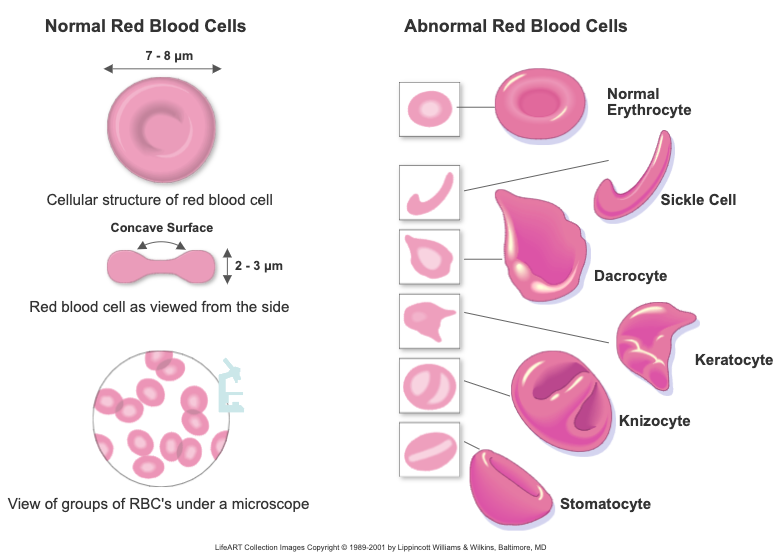
\includegraphics[width=0.9\textwidth]{images/RedBloodCellDescription.png}
\caption{\textit{An illustration of the shapes and sizes for a normal red blood cell along with the different types of abnormal red blood cells.  \cite{RedBloodCellsDescription, LifeART2000}} \label{RedBloodCell}}
\end{figure}

\noindent The RBC membrane from a mechanical perspective is perceived as a thin and highly deformable viscoelastic shell that contains a concentrated solution of haemoglobin. It behaves like an incompressible fluid with an approximate viscosity of 7 mPa s.\cite{chien1975red} The RBC membrane is critical to the deformability of RBCs as the viscoelastic properties of the protein cytoskeleton primarily influence the mechanical reaction of the RBC membrane to shear deformation.\cite{EvansE.A1976Mv} Unlike the RBC, the viscosity of the suspending medium (i.e. plasma) is usually around 1.2 mPa s and it behaves like a Newtonian fluid in micro-circulations. Given that the two primary components of blood are RBCs and plasma, the presence of RBCs is a major contributing factor to blood viscosity and hence, affecting the blood flow behaviours through extremely narrow capillaries. \\ 

\noindent In essence, the above description of the mechanical properties of RBCs summarises the essential keynotes for simulating the behaviour of RBC suspensions in micro-vascular networks under a specific given set of flow conditions. As a result, the RBCs in the simulation was modelled as a deformable capsule with a thickness of zero hyper-elastic membrane containing a viscous fluid called cytoplasm which consists of haemoglobin. In practice, these simulations are challenging due to the mechanical complexity of fluid-solid interactions especially when dealing with a large number of particles interacting among one another in a fluid.